\documentclass[a4paper,12pt]{report}
% safe参数解决与\!在内的多个冲突
% \sups命令可能被重定义,xeCJK放在tipa后
\usepackage[safe]{tipa}

% 中文支持
\usepackage[slantfont,boldfont]{xeCJK}
	\setCJKmainfont[BoldFont=SimHei,ItalicFont=KaiTi]{SimSun}
	\setCJKmathfont{STXinwei}
\usepackage{indentfirst}

% 数学环境
\usepackage{amsmath}
  \newcommand{\ue}{\mathrm{e}}
  \newcommand{\ud}{\mathop{}\negthinspace\mathrm{d}}
\usepackage{amssymb}
\usepackage{mathrsfs} % 线性代数字体
    % overline的替代命令
\newcommand{\closure}[2][3]{{}\mkern#1mu\overline{\mkern-#1mu#2}}
\usepackage{yhmath} % 左下-右上省略号
\usepackage{mathtools} % dcases环境
\usepackage{amsthm} % 定理环境
  \theoremstyle{definition}\newtheorem{laws}{Law}[section]
  \theoremstyle{plain}\newtheorem{ju}[laws]{Jury}
  \theoremstyle{remark}\newtheorem*{marg}{Margaret}
\usepackage{esint} % 多重积分,需放在amsmath后

% 下划线宏包
\usepackage{ulem}
% LaTeX符号宏包
\usepackage{hologo}
	\newcommand{\xelatex}{\Hologo{XeLaTeX}}
	\newcommand{\bibtex}{\Hologo{BibTeX}}
% 其他符号
\usepackage{wasysym}
% 带箱小页
\usepackage{boxedminipage}
% 绘图
\usepackage{tikz}
	\usetikzlibrary{calc}
	\newcommand{\tikzline}[1]{{#1\tikz{\draw[#1,line width=9](0,0)--(0.5,0);}}, }

% 奇怪的小定义
\newcommand{\dpar}{\\ \mbox{}}	% 空两行
\newcommand{\qd}[1]{{\bfseries{#1}}}	% 强调
\newcommand{\co}[1]{{\bfseries{#1}}}   % Style of concept
\newcommand{\RED}[1]{{\color{red}{#1}}}
\newcommand{\cmmd}[1]{\fbox{\texttt{\char92{}#1}}}
\newcommand{\charef}[1]{第\ref{#1}章}
\newcommand{\secref}[1]{第\ref{#1}节}
\newcommand{\pref}[1]{第\pageref{#1}页}
\newcommand{\fref}[1]{图\ref{#1}}
\newcommand{\tref}[1]{表\ref{#1}}

% 编号列表宏包,并自定义了三个列表
%\usepackage[inline]{enumitem}
%	\setlist[enumerate]{label=\arabic* - ,font=\bfseries,itemsep=0pt}
%	\setlist[itemize]{label=$\bullet$,font=\bfseries,leftmargin=\parindent}
%	\setlist[description]{font=\bfseries\uline}
%
%\newenvironment{fead}{\setlength{\parskip}{0pt}
%	\begin{description}[font=\bfseries\uline,labelindent=\parindent]
%		\setlength{\itemsep}{0pt}\setlength{\parsep}{0pt}\setlength{\parskip}{0pt}}
%	{\end{description}}
% 带宽度的
\newenvironment{para}{\setlength{\parskip}{0pt}
	\begin{description}[font=\bfseries\ttfamily]
		\setlength{\itemsep}{0pt}\setlength{\parsep}{0pt}\setlength{\parskip}{0pt}}
	{\end{description}}
\newenvironment{feae}{\setlength{\parskip}{0pt}
	\begin{enumerate}[font=\bfseries,labelindent=0pt]}
	{\end{enumerate}}
\newenvironment{feai}{\setlength{\parskip}{0pt}
	\begin{itemize}[font=\bfseries]
		\setlength{\itemsep}{0pt}\setlength{\parsep}{0pt}\setlength{\parskip}{0pt}}
	{\end{itemize}}
\newenvironment{inlinee}
{\begin{enumerate*}[label=(\arabic*), font=\rmfamily, before=\unskip{:},itemjoin={{;}},itemjoin*={{,以及:}}]}
	{\end{enumerate*}。}

% 目录和章节样式
\usepackage{titlesec}
\usepackage{titletoc}   % 用于目录

\titlecontents{chapter}[1.5em]{}
	{\contentslabel{1.5em}}{\hspace*{-2em}}{\hfill\contentspage}
	
\titlecontents{section}[3.3em]{}
	{\contentslabel{1.8em}}
	{\hspace*{-2.3em}}
	{\titlerule*[8pt]{$\cdot$}\contentspage}
%	
\titlecontents{subsection}[2.5em]{\small}
	{\thecontentslabel{} }
	{}
	{\titlerule*[5pt]{$\cdot$}\contentspage}
 %章节样式
\setcounter{secnumdepth}{3} % 一直到subsubsection
\newcommand{\chaformat}[1]{%
	\parbox[b]{.5\textwidth}{\hfill\bfseries #1}%
	\quad\rule[-12pt]{2pt}{70pt}\quad
	{\fontsize{60}{60}\selectfont\thechapter}}
\titleformat{\chapter}[block]{\hfill\LARGE\sffamily}{}{0pt}{\chaformat}[\vspace{2.5pc}\large
	\startcontents\printcontents{}{1}{\setcounter{tocdepth}{2}}]
%\titleclass{\section}{top}
%\titleformat{\section}{\Large\bfseries}{\thesection}{0.5em}{}
\titleformat*{\section}{\centering\Large\bfseries}
\titleformat{\subsubsection}[hang]{\bfseries\large}{\rule{1.5ex}{1.5ex}}{0.5em}{}
% 扩展章节
\newcommand{\starsec}{\noindent\fbox{\S\textit{注意:本章节是一个扩展阅读章节。}}
	\\ \mbox{}}

\renewcommand{\contentsname}{目录}
	\renewcommand{\tablename}{表}
	\renewcommand\arraystretch{1.2}	% 表格行距
	\renewcommand{\figurename}{图}
% 设置不需要浮动体的表格和图像标题
\setlength{\abovecaptionskip}{5pt}
\setlength{\belowcaptionskip}{3pt}
\makeatletter
\newcommand\figcaption{\def\@captype{figure}\caption}
\newcommand\tabcaption{\def\@captype{table}\caption}
\makeatother
% 图表
\usepackage{array,multirow}
  \setlength\extrarowheight{2pt} % 行高增加
\usepackage{longtable}
\usepackage{graphicx}
  \graphicspath{{./tikz/}}
% 页面修正宏包
\usepackage[top=1in]{geometry}

% 代码环境
\usepackage{listings}
% Avoid copy line numbers of the listing code (Invalid for SumatraPDF Reader)
\usepackage{accsupp}
	\newcommand{\emptyaccsupp}[1]{\BeginAccSupp{ActualText={}}#1\EndAccSupp{}}
% Color
\usepackage{xcolor}
	\definecolor{commentcolor}{RGB}{85,139,78}
	\definecolor{numbercolor}{RGB}{166,206,168}
	\definecolor{stringcolor}{RGB}{206,145,108}
	\definecolor{keywordcolor}{RGB}{34,34,250}
	\definecolor{backcolor}{RGB}{220,220,220}
	\definecolor{packagecolor}{RGB}{0,128,0}
	\definecolor{envicolor}{RGB}{185,70,15}
% LaTeX Code Style
%\lstset{language=[LaTeX]TeX,
%		basicstyle=\small\ttfamily,
%		commentstyle=\color{commentcolor},
%		keywordstyle=\color{keywordcolor},
%		stringstyle=\color{stringcolor},
%		showstringspaces=false,
%		% Package/Tikz-Lib Using
%		classoffset=0,
%		morekeywords={begin,end,usetikzlibrary},
%		keywordstyle=\color{keywordcolor},
%		classoffset=1,
%		morekeywords={article,report,book,
%			xeCJK,tikz,
%			calc},
%		keywordstyle=\color{packagecolor},
%		classoffset=2,
%		morekeywords={document,tikzpicture},
%		keywordstyle=\color{envicolor},
%		% Line Number Style
%		numbers=left,
%		numberstyle=\tiny\emptyaccsupp,
%		stepnumber=1,
%		% Frame and Background Color
%		frame=single,
%		framerule=0pt,
%		backgroundcolor=\color{backcolor},
%		% Spaces
%		% belowskip=\medskipamount,
%		emptylines=1,
%		escapeinside=``}

\lstnewenvironment{latex}[1]{\lstset{#1}}{}
\newcommand{\latexline}[1]{{\lstinline[language=TeX,basicstyle=\small\ttfamily]{#1}}}

% Tikz Code
\lstdefinelanguage{tikzlang}{
	classoffset=0, % 蓝色的keyword
	morekeywords={begin,end,newcommand,
		draw,node,coordinate,tikzstyle,foreach},
	keywordstyle=\color{keywordcolor},
	classoffset=1, % 棕色的其他关键字
	morekeywords={tikzpicture,grid,at,
		thick,thin,very,ultra,
		red,green,yellow,blue,cyan,magenta,black,
		    gray,darkgray,lightgray,brown,lime,
		    olive,orange,pink,purple,teal,violet,white},
	keywordstyle=\color{envicolor},
	morecomment=[l]{\%},
	morecomment=[s]{/*}{*/},
	morestring=[b]',
	% Escape
	escapeinside=``
}
\lstnewenvironment{tikzcode}[1]{\lstset{language=tikzlang,basicstyle=\small\ttfamily,
		breaklines=true,%backgroundcolor=\color{white},
		linewidth=0.7\linewidth,#1}}{}

% 附录
\usepackage{appendix}

% 行号
\usepackage{lineno}

% 代码输入环境
%\usepackage{verbatim,xcolor}
%\newbox\savedlines
%\newtoks\savedtokens
%\makeatletter
%\def\codeshow{%
%\global\savedtokens={}%
%\def\verbatim@processline{%
%{\setbox0=\hbox{\the\verbatim@line}%
%\hsize=\wd0
%\the\verbatim@line\par}%
%\global\savedtokens=\expandafter{\the\expandafter\savedtokens\the\verbatim@line^^J}}%
%\@tempswatrue
%\setbox0=\vbox\bgroup\parskip=0pt\topsep=0pt\partopsep=0pt
%\verbatim}
%\def\endcodeshow{\endverbatim%
%\unskip\setbox0=\lastbox\egroup
%\global\setbox\savedlines=\box0
%\addvspace{1em}\par\noindent%
%\colorbox{lightgray}{%
%\begin{minipage}{.55\textwidth}{\usebox\savedlines}\end{minipage}}%
%\hfill\fbox{\parbox{.40\textwidth}%
%{\scantokens\expandafter{\the\savedtokens\unskip\endinput}}}%
%\par\addvspace{1em}}
%\makeatother

% 引用
\usepackage[colorlinks,bookmarksopen=true,bookmarksnumbered=true]{hyperref}

%\documentclass{ctexart}
\usepackage{algorithm}
\usepackage{amsmath,bm}
\usepackage{algorithmic}
\usepackage{fancybox}
\usepackage{listings}
\usepackage{xcolor}
%\usepackage{times}
\usepackage{amssymb}
\usepackage{amsmath}
\usepackage{amsthm}
\usepackage{empheq}
\usepackage{bookman}
\usepackage{lscape}
\usepackage[framemethod=tikz]{mdframed}
\usepackage{mathtools}

\definecolor{ocre}{RGB}{243,102,25}
\definecolor{mygray}{RGB}{243,243,244}

\newcommand*\mymathbox[1]{%
  \fcolorbox{ocre}{mygray}{\hspace{1em}#1\hspace{1em}}}

\newtheoremstyle{mystyle}
  {\topsep}
  {\topsep}
  {\normalfont}
  {}
  {\sffamily\bfseries}
  {.}
  {.5em}
  {{\color{ocre}\thmname{#1}~\thmnumber{#2}}\thmnote{\,--\,#3}}%
\theoremstyle{mystyle}
\newmdtheoremenv[
  backgroundcolor=mygray,
  linecolor=ocre,
  leftmargin=20pt,
  innerleftmargin=0pt,
  innerrightmargin=0pt,
  ]{theo}{Theorem}[section]

\lstset{
columns=flexible,
numbers=left,
numberstyle=\footnotesize\color{darkgray}, 
basicstyle=\small\ttfamily,
stringstyle=\color{purple},
keywordstyle=\color[RGB]{40,40,255}\bfseries,
commentstyle=\it\color[RGB]{0,96,96},  
stringstyle=\rmfamily\slshape\color[RGB]{128,0,0}, 
showstringspaces=false,      
% directivestyle=\color{blue},
frame=shadowbox,
%framerule=0pt,
backgroundcolor=\color[RGB]{245,245,244},
escapeinside=``, %逃逸字符(1左面的键),用于显示中文
breaklines,
extendedchars=false,
%解决代码跨页时,章节标题,页眉等汉字不显示的问题
xleftmargin=2em,xrightmargin=2em,
aboveskip=1em,%设置边距
tabsize=4, %设置tab空格数  
showspaces=false %不显示空格 
rulesepcolor=\color{red!20!green!20!blue!20}
%rulesepcolor=\color{brown}
}


\title{数值分析第二次大作业}
\author{张晋\\学号:15091060}
\date{最后更新于:\today}
\begin{document}

\maketitle

\tableofcontents


\newpage

\chapter{题目}
试求矩阵$\bm{A}=\big[\,a_{ij}\,\big]_{10\times 10}$的全部特征值,
并对其中的每一个特征值求相应的特征向量,已知:
\begin{equation*}
a_{ij}=\begin{cases}
\text{sin}(0.5i+0.2j)& i\neq j \\
1.52\text{cos}(i+1.2j) & i=j
\end{cases} \qquad (i,j=1,2,\cdots,10)
\end{equation*}

\qd{说明}:
\begin{enumerate}
\item 用双步位移QR法求矩阵特征值时,要求迭代精度水平为$\epsilon=10^{-12}$。

\item 打印以下内容:

\begin{enumerate}
\item 全部源程序;

\item 矩阵$\bm{A}$经过拟上三角化后所得的拟上三角阵
$\bm{A}^{(n-1)}$;

\item 对矩阵$\bm{A}^{(n-1)}$使用双步位移QR法迭代
结束后所得的矩阵$\bm{Q}$和$\bm{R}$,
并把$R\times Q$打印,看是不是拟上三角阵;

\item 矩阵$\bm{A}$的全部特征值$\lambda_{i}=(R_i,I_i)\qquad (i=1,2,\cdots ,10)$;

\item 矩阵$\bm{A}$相对应于实特征值的特征向量。
\end{enumerate}
\item 采用e型输出实型数,并且至少显示12位有效数字。
\end{enumerate}



\newpage
\chapter{算法设计方案}
\section{Householder变换}

\begin{theo}
我们称矩阵
\begin{equation}
H=I-2vv^{\ast},\qquad v\in\mathbb{C}^n\quad s.t.
\quad ||v||_2=\sqrt{v^{\ast}v}=1,
\end{equation}
为\qd{Householder矩阵}(或Householder变换),
向量$v$称为\qd{Householder向量}.
我们通常将矩阵记为$H(v)$。
\end{theo}

Householder变换又称为反射变换或镜像变换,有明显的几何意义。在
$\mathbb{R}^3$中,给定一个向量$\alpha$,令$\beta$表示$\alpha$关于平面$\pi$(以$\omega$为法向量)的反射变换所得像,如图所示,

记
\[\omega  = \frac{{\alpha  - \beta }}{{\left| {\alpha  - \beta } \right|}} \in {\mathbb{R}^3}\]
\[H(\omega ) = I - 2\omega {\omega ^T}\]

则$H(\omega )\alpha  = \beta $

即:该变换将向量$\alpha$变成了以$\beta$为法向量的平面的对称向量$\beta$。因此,Householder 变换也称为反射变换.
\newpage
下面是关于 Householder 矩阵的几个基本性质.
\begin{theo}
设$H\in \mathbb{C}^{n\times n}$是一个$Householder$矩阵,
则

(1) $H^{\ast}=H$, 即$H$是Hermite的;

(2) $H^{\ast}H=I$, 即$H$是酉矩阵;

(3) $H^{2}=I$, 所以$H^{-1} = H$;

(4) $det(H) = −1$;

(5) $H$有两个互异的特征值:$\lambda= 1,\lambda= −1$,
其中$\lambda=1$的代数重数为$n − 1$.
\end{theo}

\begin{figure}[ht]
\small
\centering
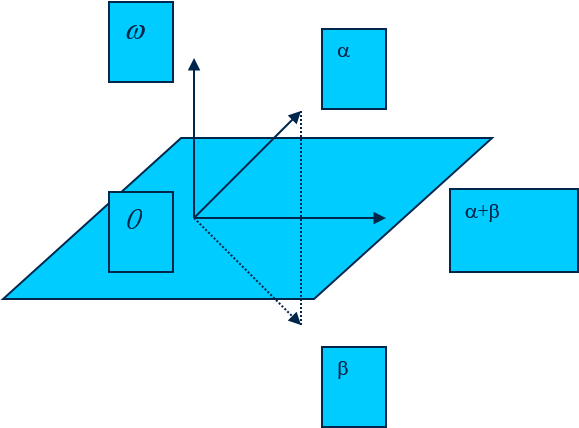
\includegraphics[width=12cm]{1.png}
\caption{Householder} \label{fig:1}
\end{figure}

\newpage
\section{QR分解}
QR分解也称为正交三角分解

QR分解将一个矩阵分解一个正交矩阵 (酉矩阵) 和一个三角矩阵的乘积. QR分解被广泛应
用于线性最小二乘问题的求解和矩阵特征值的计算

\begin{algorithm}[h]  
\caption{QR Iteration}  
\begin{algorithmic}[1]  
\STATE Set $A_1=A$ and $k=1$
\WHILE {not convergence}
\STATE ${A_{k}} = Q_k R_k$
\STATE Compute $A_{k+1}=R_k Q_k$
\STATE k=k+1
\ENDWHILE
\end{algorithmic}  
\end{algorithm}  

在 QR 迭代算法中, 我们有
\[
A_{k+1}=R_kQ_k=(Q_k^TQ_k)R_kQ_k=Q^T_k(Q_kR_k)Q_k=Q_k^TA_kQ_k\]
由这个递推关系可得
\begin{align*}
A_{k+1}=Q_k^TA_kQ_k&=Q^T_kQ^T_{k-1}A_{k-1}Q_{k-1}Q_k\\
&=\cdots\\
&=Q^T_kQ^T_{k-1}\cdots Q^T_1AQ_1\cdots Q_{k-1}Q_k.
\end{align*}

记\boxed{{\tilde Q}_k=Q_1\cdots Q_{k-1}Q_k},则
\[A_{k+1}={\tilde Q}_k^TA{\tilde Q}_k\]
即$A_{k+1}$于$A$正交相似

\begin{theo}[QR 迭代的收敛性]
设$A=VJV^{-1}\in \mathbb{R}^{n\times n}$,
其中$J=diag(\lambda_1,\lambda_2,\cdots,\lambda_n)$,
且$|\lambda_1|>|\lambda_2|>\cdots>|\lambda_n|$。
若$V^{-1}$的所有主子矩阵都非奇异(即$V^{-1}$存在$LU$分解),
则$A_k$的对角线以下的元素均收敛到0.
\end{theo}

\newpage
\section{带位移的QR迭代}
为了加快$QR$迭代的收敛速度, 我们可以采用位移策略和反迭代思想.
\begin{algorithm}[h]  
\caption{QR Iteration with shift}  
\begin{algorithmic}[1]  
\STATE Set $A_1=A$ and $k=1$
\WHILE {not convergence}
\STATE Choose a shift $\sigma_k$
\STATE ${A_{k}-\sigma_kI} = Q_k R_k$
\STATE Compute $A_{k+1}=R_k Q_k+\sigma_kI$
\STATE k=k+1
\ENDWHILE
\end{algorithmic}  
\end{algorithm}  

我们有
\begin{align*}
A_{k+1}=R_kQ_k+\sigma_kI&=(Q^T_kQ_k)R_kQ_k+\sigma_kI\\
&=Q^T_k(A_k-\sigma_kI)Q_k+\sigma_kI\\
&=Q^T_kA_kQ_k
\end{align*}

所以, 带位移的$QR$算法中所得到的所有矩阵$A_k$都与$A$正交相似.

\newpage
\chapter{问题求解}
\begin{enumerate}
\item 初始化定义$A$矩阵

\item 采用$Householder$变化将$A$矩阵拟上三角化得到矩阵$A^{n-1}$

\item 采用$QR$分解将矩阵$A^{n-1}$分解为矩阵Q与R,并打印RQ

\item 用带双步位移的QR方法求解所有特征值

\item 用Gauss消去法求解$(A-\lambda I)X=0$,得到对应的特征向量

\item 输出
\end{enumerate}
\newpage
\begin{figure}[ht]
\small
\centering
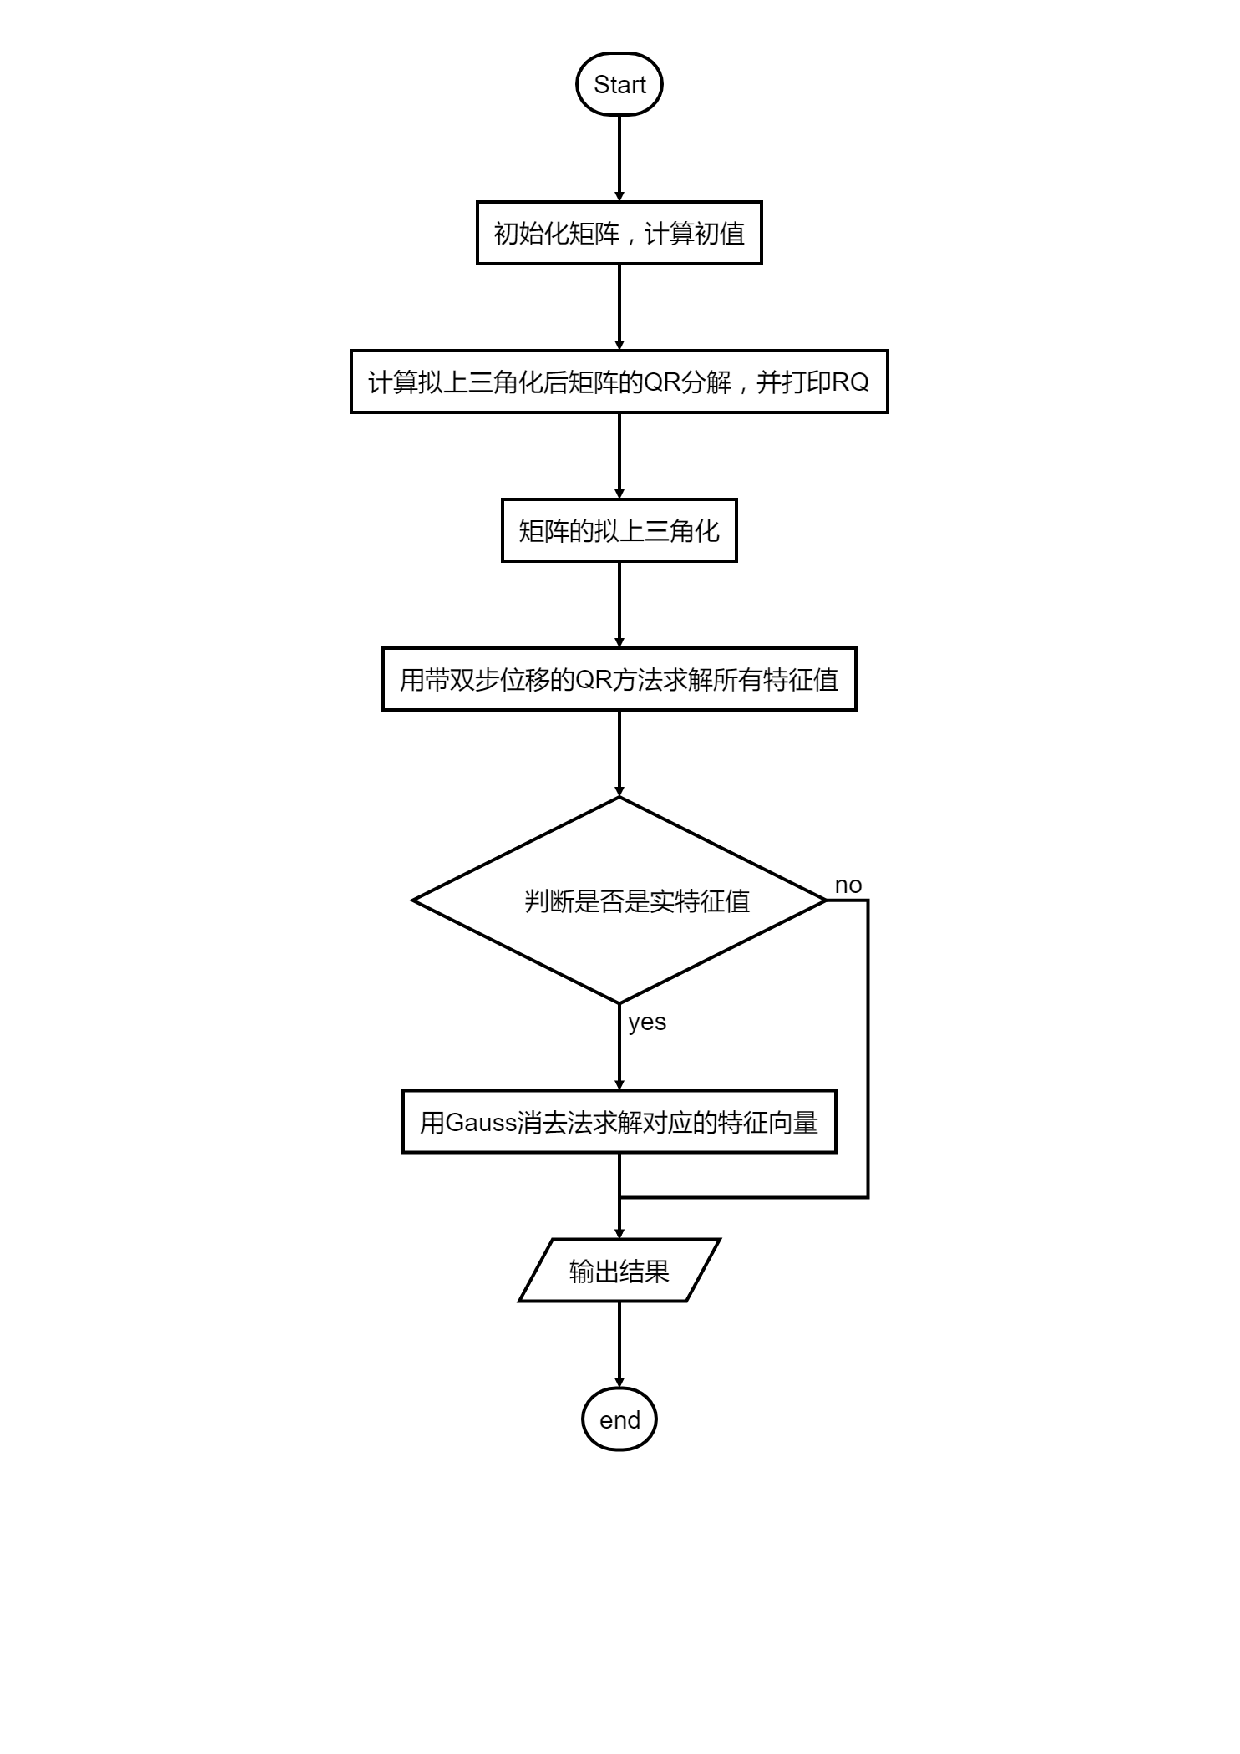
\includegraphics[width=10cm]{2.pdf}
\caption{流程图} \label{fig:1}
\end{figure}

\chapter{源程序}
\section{C语言版大作业}
\begin{lstlisting}[language=C]
#include<stdio.h>
#include<math.h>
#include<string.h>
#define N 20
const double eps=1e-12;
double a[N][N],B[N][N],C[N][N];
int n=10;

typedef struct{
//定义复数结构体
    double Re;
    double Im;
}ComplexNumber;

void zeroMat(double a[N][N]){
    for(int i= 1; i<=10; i++) {
        for(int j = 1; j<=10; j++) {
            if (fabs(a[i][j])<eps)
                a[i][j] = 0;
        }
    }
}

void def(){
	//初始化A数组
	for(int i=1;i<=n;i++)
		for(int j=1;j<=n;j++){
			if(i==j)
				a[i][j]=1.52*cos(i+1.2*j);
			else if(i!=j)
				a[i][j]=sin(0.5*i+0.2*j);
		}
}

void eye(double Q[N][N]){
	//定义单位阵 
	for(int i=1;i<=n;i++)
		for(int j=1;j<=n;j++)
			Q[i][j]=(i==j);
}

int Is_zero(double Q[N][N],int r,int k){
	//K>0表示在QR中调用,K<0表示在 DQR中调用 
	int kk=n;//更改数组大小 
	if(k<0){kk=-k;k=1;}
	for(int i=r+k;i<=kk;i++)
		if(fabs(Q[i][r])>eps)
			return 0;
	return 1;
}


int sgn(double x){
	if(x>0)
		return 1;
	return -1;
}

void Matirix_M(double A[N][N],double x[N],double y[N],double h){
	for(int i=1;i<=n;i++)y[i]=0;
	for(int i=1;i<=n;i++)
		for(int j=1;j<=n;j++)
			y[i]+=A[i][j]*x[j]/h;
}

double Vector_M(double x[N],double y[N]){
	double sum=0;
	for(int i=1;i<=n;i++)
		sum+=x[i]*y[i];
	return sum;
}

void MatirixM_M(double X[N][N],double Y[N][N]){
	for(int i=1;i<=n;i++)
		for(int j=1;j<=n;j++)
			for(int k=1;k<=n;k++)
				B[i][j]+=X[i][k]*Y[k][j];
}

void copy(double X[N][N],double Y[N][N]){
	for(int i=1;i<=n;i++)
		for(int j=1;j<=n;j++)
			X[i][j]=Y[i][j];
}

void output(double A[N][N]){
	for(int i=1;i<=n;i++){
		for(int j=1;j<=n;j++)
			printf("%.12e ",A[i][j]);
		printf("\n");
	}
}

void QR(double A[N][N],double Q[N][N]){
	double u[N],w[N],p[N],d,c,h;
	eye(Q);
	for(int r=1;r<n;r++){
		d=0;
		if(Is_zero(A,r,1))continue;
		for(int i=r;i<=n;i++)
			d+=A[i][r]*A[i][r];
		d=sqrt(d);
		c=-sgn(A[r][r])*d;
		h=c*c-c*A[r][r];
		for(int i=1;i<=n;i++){
			if(i<r)
				u[i]=0;
			else if(i==r)
				u[i]=A[r][r]-c;
			else if(i>r)
				u[i]=A[i][r];
		}
		memset(w,0,sizeof(w));
		Matirix_M(Q,u,w,1);
		for(int i=1;i<=n;i++)
			for(int j=1;j<=n;j++)
				Q[i][j]-=(w[i]*u[j]/h);
		memset(p,0,sizeof(p));
		for(int i=1;i<=n;i++)
			for(int j=1;j<=n;j++)
				p[i]+=(A[j][i]*u[j]/h);
		for(int i=1;i<=n;i++)
			for(int j=1;j<=n;j++)
				A[i][j]-=(u[i]*p[j]);
	}
}

void Householder_Triangularization(double A[N][N]){
	double u[N],p[N],q[N],d,c,h;
	for(int r=1;r<n-1;r++){
		d=0;
		if(Is_zero(A,r,2))continue;
		for(int i=r+1;i<=n;i++)
			d+=A[i][r]*A[i][r];
		d=sqrt(d);
		c=-sgn(A[r+1][r])*d;
		h=c*c-c*A[r+1][r];
		for(int i=1;i<=n;i++){
			if(i<=r)
				u[i]=0;
			else if(i==(r+1))
				u[i]=A[i][r]-c;
			else if(i>r)
				u[i]=A[i][r];
		}
		memset(p,0,sizeof(p));
		for(int i=1;i<=n;i++)
			for(int j=1;j<=n;j++)
				p[i]+=(A[j][i]*u[j]/h);
		Matirix_M(A,u,q,h);
		c=Vector_M(p,u)/h;
		for(int i=1;i<=n;i++)
			q[i]-=u[i]*c;
		for(int i=1;i<=n;i++)
			for(int j=1;j<=n;j++)
				A[i][j]-=(q[i]*u[j]+u[i]*p[j]);
	}
}


void select(int k,double b[N][N]){
	double max,c;
	int m=k;
	max=b[k][k];
	for(int i=k+1;i<=n;i++)
		if(fabs(b[i][k])>fabs(max)){
			max=b[i][k];
			m=i;
		}
	if(m!=k)
		for(int i=k;i<=n+1;i++){
		c=b[m][i];
		b[m][i]=b[k][i];
		b[k][i]=c;
		}
}

//Gauss消元法
void gauss(double lambda)
{
    double X[N];
    double m,sum,t;
    def();
    memset(X,0,sizeof(X));
    for(int i=1;i<=n;i++){
        a[i][i]-=lambda;
        a[i][n+1]=0;
    }
	for(int k=1;k<n;k++){
		select(k,a);
		for(int i=k+1;i<=n;i++){
			m=a[i][k]/a[k][k];
		for(int j=k;j<=n+1;j++)
			a[i][j]-=m*a[k][j];
		}	
	}
	X[n]=1;
	for(int i=n-1;i>=1;i--){
		sum=0;	
		for(int j=i+1;j<=n;j++) 
			sum+=a[i][j]*X[j];
		if(fabs(a[i][i])>eps)
			X[i]=(a[i][n+1]-sum)/a[i][i];
		else
			X[i]=0;
	}
	t=0;
	for(int i=1;i<=n;i++)
		t+=X[i]*X[i];
	t=sqrt(t);
	printf("Eigenvector=(");
	for(int i=1;i<=n;i++)
        printf("%lf ", X[i]/t);
    printf(")\n");
}

void DQR(double A[N][N]){
	double Q[N][N],M[N][N],s,t,re,im,a,b,c,d;
	double u[N],v[N],p[N],q[N],h,det;
	ComplexNumber L[N]; 
	int m=n,LL=1000,r=1;
	for(int k=1;k<=100;k++){
		if (m == 1) {
            L[r].Re = A[m][m];
            L[r].Im = 0; break;
        }
        else if(m<=0)break; 
		if(fabs(A[m][m-1])<=eps){
			L[r].Re = A[m][m];
            L[r].Im = 0;
            m--;r++;continue;
		}
		a=A[m-1][m-1];
		b=A[m-1][m];
		c=A[m][m-1];
		d=A[m][m];
		re=(a+d)/2;
		det=(a-d)*(a-d)+4*b*c;
		
		if((m==2)||(fabs(A[m-1][m-2])<=eps)){
			if(det>0){
				L[r].Re = re+sqrt(det)/2;
            	L[r].Im = 0;
            	L[r+1].Re = re-sqrt(det)/2;
            	L[r+1].Im = 0;
            }
            else if(det<0){
            	L[r].Re = re;
            	L[r].Im=sqrt(fabs(det))/2;
            	L[r+1].Re = re;
            	L[r+1].Im = -L[r].Im;
			}
            m-=2;
			r+=2;
			continue;
		}
		if(k==LL)break;
		s=a+d;
		t=a*d-c*b;
		memset(M,0,sizeof(M));
		for(int i=1;i<=m;i++)
			for(int j=1;j<=m;j++){
				for(int l=1;l<=m;l++)
					M[i][j]+=A[i][l]*A[l][j];
				M[i][j] -= s*A[i][j];
				M[i][j] += t*(i==j);
			}

		for(int r=1;r<m;r++){
			d=0;
			if(Is_zero(M,r,-m))continue;
			for(int i=r;i<=m;i++)
				d+=M[i][r]*M[i][r];
			d=sqrt(d);
			c=-sgn(M[r][r])*d;
			h=c*c-c*M[r][r];
			for(int i=1;i<=m;i++){
				if(i<r)
					u[i]=0;
				else if(i==r)
					u[i]=M[r][r]-c;
				else if(i>r)
					u[i]=M[i][r];
			}
			memset(p,0,sizeof(p));
			memset(q,0,sizeof(q));
			memset(v,0,sizeof(v));
			for(int i=1;i<=m;i++)
				for(int j=1;j<=m;j++)
					v[i]+=(M[j][i]*u[j]/h);	
			for(int i=1;i<=m;i++)
				for(int j=1;j<=m;j++){
					M[i][j]-=(u[i]*v[j]);
					p[i]+=(A[j][i]*u[j]/h);
					q[i]+=(A[i][j]*u[j]/h);
				}

			c=0;
			for(int i=1;i<=m;i++)
				c+=p[i]*u[i]/h;
			for(int i=1;i<=m;i++)
				q[i]-=u[i]*c;
			for(int i=1;i<=m;i++)
				for(int j=1;j<=m;j++)
					A[i][j]-=(q[i]*u[j]+u[i]*p[j]);
			zeroMat(A);
		}

	}
	zeroMat(A);
 	for(int r = 1; r<=10; r++){
        printf("\n");
        if (L[r].Im == 0) {
            printf("lambda[%d] = %.12e \n", r , L[r].Re); 
            gauss(L[r].Re);
        }
        else {
            printf("lambda[%d] = %.12e + i*%.12e\n", r , L[r].Re, L[r].Im);
        }
    }	
}

int main(){
	double Q[N][N];
	freopen("Works.in","r",stdin);
	freopen("Works.out","w",stdout);
	def();
	Householder_Triangularization(a);
	printf("A_n-1:\n");
	output(a);
	QR(a,Q);
	printf("\nR:\n");
	output(a);
	printf("\nQ:\n");
	output(Q);
	memset(B,0,sizeof(B));
	MatirixM_M(a,Q);
	printf("\nR*Q:\n");
	output(B);
	def();
	DQR(a);
	return 0;
}
\end{lstlisting}


\newpage
\section{MATLAB版QR分解}
\begin{lstlisting}[language=Octave]
%fid=fopen('A_out.txt','w');
A=[
-0.894522	-0.099331	-1.099832	-0.766504	0.170760	-1.934883	-0.083902	0.913257	-0.640798	0.194673;	
-2.347878	2.372058	1.827999	0.326656	0.208236	2.088987	0.184786	-1.263015	0.679069	-0.467215;	
0.000000	1.735954	-1.165023	-1.246744	-0.629823	-1.984820	0.297575	0.633930	-0.130852	0.304030;	
0.000000	0.000000	-1.292938	-1.126239	1.190783	-1.308773	0.186015	0.423673	-0.101960	0.194366;	
0.000000	0.000000	0.000000	1.577711	0.816936	0.446153	-0.043651	-0.466598	0.294123	-0.103442;	
0.000000	0.000000	-0.000000	0.000000	-0.772898	-1.601028	-0.291269	-0.243434	0.673629	0.262477;	
0.000000	0.000000	0.000000	0.000000	-0.000000	-0.729677	-0.007965	0.971074	-0.129897	0.027802;	
0.000000	0.000000	-0.000000	0.000000	-0.000000	0.000000	0.794554	-0.452514	0.504890	-0.121121;	
0.000000	0.000000	0.000000	0.000000	-0.000000	0.000000	-0.000000	0.703991	0.126754	-0.371470;	
0.000000	0.000000	0.000000	0.000000	-0.000000	0.000000	0.000000	0.000000	-0.491959	0.408151;
];
for i=1:5
[q,r]=qr(A);
r
A=r*q;
end
A
r
q
e=diag(A)
eig(A)
%fclose(fid);
\end{lstlisting}


\chapter{计算结果}
后面为输出结果:
\newpage
\begin{landscape}
\small

$A_{n-1}$
$1\sim$5列:
\[
\begin{matrix}
-8.945216982281e-001 & -9.933136491826e-002 & -1.099831758877e+000 & -7.665038709077e-001 & 1.707601141456e-001\\-2.347878362416e+000 & 2.372057921598e+000 & 1.827998552316e+000 & 3.266556884714e-001 & 2.082360583635e-001\\0.000000000000e+000 & 1.735954469946e+000 & -1.165023367477e+000 & -1.246744443518e+000 & -6.298225489084e-001\\0.000000000000e+000 & 0.000000000000e+000 & -1.292937563924e+000 & -1.126239225902e+000 & 1.190782911924e+000\\0.000000000000e+000 & 0.000000000000e+000 & 8.357856452328e-017 & 1.577711153032e+000 & 8.169358328160e-001\\0.000000000000e+000 & 0.000000000000e+000 & -9.764615357502e-017 & 0.000000000000e+000 & -7.728975134989e-001\\0.000000000000e+000 & 0.000000000000e+000 & 5.527597418716e-017 & 0.000000000000e+000 & -6.046925797698e-017\\0.000000000000e+000 & 0.000000000000e+000 & -1.453366930807e-016 & 0.000000000000e+000 & -2.216961051353e-017\\0.000000000000e+000 & 0.000000000000e+000 & 7.284428787973e-017 & 0.000000000000e+000 & -8.264895477591e-018\\0.000000000000e+000 & 0.000000000000e+000 & 1.475442153596e-017 & 0.000000000000e+000 & -1.196693128035e-016\\
\end{matrix}\]

$A_{n-1}$
$6\sim$10列:
\[
\begin{matrix}
-1.934882558889e+000 & -8.390208705246e-002 & 9.132565113143e-001 & -6.407977009188e-001 & 1.946733678685e-001\\2.088987009941e+000 & 1.847861910289e-001 & -1.263015266080e+000 & 6.790694668499e-001 & -4.672150886500e-001\\-1.984820180992e+000 & 2.975750060800e-001 & 6.339300596595e-001 & -1.308518928772e-001 & 3.040301036095e-001\\-1.308772983895e+000 & 1.860151662666e-001 & 4.236733936881e-001 & -1.019600826545e-001 & 1.943660914505e-001\\4.461531723828e-001 & -4.365092541609e-002 & -4.665979167188e-001 & 2.941231566184e-001 & -1.034421113665e-001\\-1.601028244046e+000 & -2.912685474827e-001 & -2.434337858321e-001 & 6.736286084510e-001 & 2.624772904937e-001\\-7.296773946362e-001 & -7.965456279819e-003 & 9.710739102007e-001 & -1.298967368574e-001 & 2.780242081241e-002\\0.000000000000e+000 & 7.945539612976e-001 & -4.525143454606e-001 & 5.048901527575e-001 & -1.211210193512e-001\\0.000000000000e+000 & -1.819189274915e-016 & 7.039911373514e-001 & 1.267535523498e-001 & -3.714696735513e-001\\0.000000000000e+000 & 1.280699160267e-016 & 0.000000000000e+000 & -4.919586872214e-001 & 4.081509766399e-001\\
\end{matrix}\]


\newpage
$R\,1\sim 5$列:
\[
\begin{matrix}
2.512509079248e+000 & -2.181265513645e+000 & -1.316649918648e+000 & -3.235549645996e-002 & -2.553867638933e-001\\0.000000000000e+000 & -1.972851789714e+000 & 2.276016623827e-001 & 7.014634531795e-001 & 5.947854062317e-001\\0.000000000000e+000 & 0.000000000000e+000 & 2.407240343439e+000 & 1.722528346094e+000 & -4.505704077291e-001\\0.000000000000e+000 & 0.000000000000e+000 & 0.000000000000e+000 & 1.595615664669e+000 & 6.397406649436e-001\\0.000000000000e+000 & 0.000000000000e+000 & 0.000000000000e+000 & 0.000000000000e+000 & -1.456242593458e+000\\0.000000000000e+000 & 0.000000000000e+000 & 0.000000000000e+000 & 0.000000000000e+000 & 8.975288153029e-017\\0.000000000000e+000 & 0.000000000000e+000 & 0.000000000000e+000 & 0.000000000000e+000 & -7.745003985679e-018\\0.000000000000e+000 & 0.000000000000e+000 & 0.000000000000e+000 & 0.000000000000e+000 & 5.471400724120e-017\\0.000000000000e+000 & 0.000000000000e+000 & 0.000000000000e+000 & 0.000000000000e+000 & 2.321397713515e-017\\0.000000000000e+000 & 0.000000000000e+000 & 0.000000000000e+000 & 0.000000000000e+000 & -2.603604216329e-017\\
\end{matrix}\]

$R$
$6\sim$10列:
\[
\begin{matrix}
-1.263236417243e+000 & -1.428067524844e-001 & 8.551127106196e-001 & -4.064323860885e-001 & 3.672920640297e-001\\5.340587633903e-001 & -3.303516655914e-001 & 6.131164883828e-002 & -2.842350072136e-001 & -1.020581006877e-001\\3.392449531044e+000 & -1.121444617851e-001 & -1.448802456850e+000 & 7.311045593936e-001 & -4.847285804893e-001\\3.502375215214e-001 & -6.543701621428e-002 & -3.985833699409e-001 & 2.393366716784e-001 & -9.059576583919e-002\\-1.416208323337e+000 & -2.740258546573e-001 & 2.820474174287e-001 & 3.146375562716e-002 & 2.179593898341e-001\\1.239676225669e+000 & 1.437893689789e-001 & -1.965876544047e-001 & -5.501588373900e-001 & -1.563867947060e-001\\0.000000000000e+000 & -8.001939216933e-001 & 3.239240677887e-001 & -4.348133701956e-001 & 1.296863513999e-001\\0.000000000000e+000 & 0.000000000000e+000 & 1.309558711582e+000 & -4.522300337931e-001 & -2.541297741346e-001\\0.000000000000e+000 & 0.000000000000e+000 & 7.388504903301e-017 & -6.591084569144e-001 & 4.900007103780e-001\\0.000000000000e+000 & 0.000000000000e+000 & -8.286706929455e-017 & 0.000000000000e+000 & 6.373330490059e-002\\
\end{matrix}\]

\newpage
$Q\,1\sim 5$列:
\[
\begin{matrix}
-3.560272500571e-001 & 4.439873952785e-001 & -6.935939248834e-001 & 6.597513287486e-002 & 3.701042887335e-001\\-9.344755733655e-001 & -1.691554235406e-001 & 2.642533895704e-001 & -2.513596481179e-002 & -1.410065879813e-001\\0.000000000000e+000 & -8.799213803066e-001 & -4.007708665994e-001 & 3.812160145536e-002 & 2.138528196492e-001\\0.000000000000e+000 & 0.000000000000e+000 & -5.371036454452e-001 & -1.260096502461e-001 & -7.068831837949e-001\\0.000000000000e+000 & 0.000000000000e+000 & 3.471965927751e-017 & 9.887789321494e-001 & -1.266092216426e-001\\0.000000000000e+000 & 0.000000000000e+000 & -4.056352488489e-017 & 4.378988184867e-017 & 5.307477730505e-001\\0.000000000000e+000 & 0.000000000000e+000 & 2.296238277072e-017 & -2.478877344479e-017 & 2.352952836071e-017\\0.000000000000e+000 & 0.000000000000e+000 & -6.037481611537e-017 & 6.517693104408e-017 & 6.253700423368e-017\\0.000000000000e+000 & 0.000000000000e+000 & 3.026049645531e-017 & -3.266736725224e-017 & -1.803836264252e-017\\0.000000000000e+000 & 0.000000000000e+000 & 6.129185054653e-018 & -6.616690490620e-018 & 7.737359003671e-017\\
\end{matrix}\]

$Q\,6\sim 10$列:
\[
\begin{matrix}
1.873680253022e-001 & -1.616846253861e-002 & 1.142209065421e-001 & 4.846147534278e-002 & -5.435281546003e-002\\-7.138562494120e-002 & 6.160046789174e-003 & -4.351719447171e-002 & -1.846341016476e-002 & 2.070796067082e-002\\1.082645668876e-001 & -9.342424307229e-003 & 6.599886483483e-002 & 2.800189963180e-002 & -3.140602039975e-002\\-3.578648243181e-001 & 3.088106413322e-002 & -2.181569912327e-001 & -9.255932185744e-002 & 1.038115266702e-001\\-6.409685206678e-002 & 5.531080075230e-003 & -3.907390568777e-002 & -1.657821824708e-002 & 1.859359069582e-002\\-6.851618290904e-001 & 5.912435352117e-002 & -4.176796180699e-001 & -1.772124834679e-001 & 1.987557610042e-001\\-5.886032010032e-001 & -9.581355780502e-002 & 6.768677853804e-001 & 2.871804513252e-001 & -3.220922591440e-001\\2.182477409330e-016 & -9.929517580142e-001 & -9.993700299902e-002 & -4.240112211755e-002 & 4.755572027991e-002\\-9.418745488859e-017 & 2.150264502325e-016 & 5.375789043480e-001 & -5.611563234389e-001 & 6.293746914713e-001\\7.348820816588e-017 & -1.736576984577e-016 & 4.208932092508e-017 & 7.464002047925e-001 & 6.654973585866e-001\\
\end{matrix}\]

\newpage
$R\ast Q\,1\sim 5$列:
\[
\begin{matrix}
1.143817643298e+000 & 2.643043667321e+000 & -1.774014655111e+000 & -7.804541680122e-002 & 3.406398561353e-001\\1.843581807358e+000 & 1.334470111482e-001 & -9.893074658739e-001 & 5.579861874654e-001 & 3.915081963850e-002\\0.000000000000e+000 & -2.118182245729e+000 & -1.889928052623e+000 & -5.708018640629e-001 & 1.154750215959e+000\\0.000000000000e+000 & 0.000000000000e+000 & -8.570109902230e-001 & 4.314991197035e-001 & -1.023023164209e+000\\0.000000000000e+000 & 0.000000000000e+000 & -1.414667033083e-017 & -1.439901996509e+000 & -5.672756725063e-001\\0.000000000000e+000 & 0.000000000000e+000 & -5.272155056859e-017 & 1.456606955283e-016 & 6.579553960773e-001\\0.000000000000e+000 & 0.000000000000e+000 & -5.029401194954e-017 & 4.663621929838e-017 & 2.028726399036e-017\\0.000000000000e+000 & 0.000000000000e+000 & -9.430668015218e-017 & 1.559077381528e-016 & 6.346313720807e-017\\0.000000000000e+000 & 0.000000000000e+000 & -1.694164409331e-017 & 4.124264650296e-017 & 4.686324787275e-017\\0.000000000000e+000 & 0.000000000000e+000 & 3.906332198803e-019 & -2.616559352009e-017 & 8.227677638012e-018\\
\end{matrix}\]

$R\ast Q\,6\sim 10$列:
\[
\begin{matrix}
1.461454600932e+000 & -9.542620239375e-001 & 4.390636920106e-001 & 7.812046500198e-001 & -3.242676232229e-001\\-2.951491456489e-001 & 1.302107099262e-002 & -6.809912257186e-001 & -1.407766316366e-001 & 4.534362093239e-003\\-2.585301662617e+000 & 1.678124198417e+000 & -1.154349560089e+000 & -1.428583810585e+000 & 8.738827597003e-001\\-8.134730259318e-001 & 4.755641447902e-001 & -3.951755882759e-001 & -4.241791598500e-001 & 3.396131374910e-001\\1.224964946486e+000 & -3.455910828759e-001 & 4.516704416505e-001 & 3.294865537961e-001 & -4.202787739855e-002\\-9.340137131103e-001 & 2.547201414468e-001 & -6.965685047393e-001 & 2.194090527527e-002 & -2.596005659042e-001\\4.709967037320e-001 & -2.449715460025e-001 & -8.077439833310e-001 & 9.726139591002e-002 & 8.578610393813e-002\\3.062200889581e-016 & -1.300328624888e+000 & -3.739826989665e-001 & 8.562468804235e-003 & -3.914678236392e-001\\9.660107939969e-017 & -3.000540383773e-016 & -3.543228021145e-001 & 7.355995090042e-001 & -8.873200325455e-002\\6.352474720579e-018 & 7.107121565932e-017 & 1.198130793216e-017 & 4.757055182990e-002 & 4.241434606534e-002\\
\end{matrix}\]



\newpage
特征值与向量如下:

$\lambda_{1}= 9.432879572769e-001$ 

Eigenvector=(0.079620,\quad 0.045421,\quad -0.018272,\quad -0.047961,\quad -0.349567,\quad 0.207215,\quad -0.152312,\quad 0.820634,\quad -0.355466,\quad 0.028866)


\vbox{}
$\lambda_{2}= 6.489488202110e-001$ 

Eigenvector=(0.108435,\quad 0.071344,\quad 0.382502,\quad -0.047100,\quad -0.717804,\quad 0.181519,\quad -0.226006,\quad 0.388381,\quad 0.289696,\quad 0.024333)


\vbox{}
$\lambda_{3}= -9.891143464725e-001$+ i*1.084758631513e-001


\vbox{}
$\lambda_{4}= -9.891143464725e-001$- i*1.084758631513e-001


\vbox{}
$\lambda_{5}= 4.954990923624e-002$ 

Eigenvector=(-0.213768,\quad -0.206774,\quad 0.386829,\quad -0.031112,\quad -0.380939,\quad -0.125174,\quad 0.644716,\quad -0.308201,\quad -0.295977,\quad 0.043723)


\vbox{}
$\lambda_{6}= -1.493147080915e+000$ 

Eigenvector=(-0.561341,\quad 0.778192,\quad 0.014364,\quad -0.277602,\quad 0.003568,\quad -0.002548,\quad -0.022061,\quad -0.011758,\quad -0.013173,\quad 0.035016)


\vbox{}
$\lambda_{7}= 1.590313458807e+000$ 

Eigenvector=(0.062377,\quad -0.011231,\quad -0.252846,\quad -0.130988,\quad -0.381985,\quad 0.815575,\quad -0.123377,\quad -0.067721,\quad 0.271945,\quad 0.100282)


\vbox{}
$\lambda_{8}= -2.336865932238e+000$+ i*8.934379210213e-001


\vbox{}
$\lambda_{9}= -2.336865932238e+000$- i*8.934379210213e-001


\vbox{}
$\lambda_{10}= 3.389613438816e+000$ 

Eigenvector=(-0.104872,\quad -0.217677,\quad -0.474694,\quad -0.259384,\quad -0.304665,\quad -0.259452,\quad 0.086866,\quad 0.405258,\quad 0.509628,\quad 0.239515)
\end{landscape}
\chapter{讨论}
\normalsize
1.在对$n\times n$实矩阵$\bm{A}$作QR分解或双步位移分解时不需要形成具体的矩阵$\bm{H}_i$,这样可以避免矩阵与矩阵相乘,大大减少了计算量。

2.在QR分解中,R矩阵可以直接储存在A的上三角部分,而在$M_k$的QR分解中,不需要再生成$\bm{B},\bm{C}$矩阵,直接在$\bm{M},\bm{A}$矩阵中迭代即可,以节约储存空间。

3.QR方法适用于计算一般实矩阵的全部特征值,但对于大型实矩阵,则收敛速度不够用了,这时我们为了加速收敛,可以引入位移量,通常, 位移越离特征值越近,收敛速度就越快,如果位移$\sigma$与某个特征值非常接近, 则$\bm{A}_{n,n}^{(k)}-\sigma$就非常接近于0.
这说明$\bm{A}_{n,n}^{(k)}$通常会首先收敛到$\bm{A}$的一个特征值.所以令$\sigma=\bm{A}_{n,n}^{(k)}$是一个不错的选择.
但是, 如果这个特征值是复数, 这种位移选取方法就可能失效.

假设$\sigma \in \mathbb{C}$是 $\bm{A}$ 的某个复特征值 $\lambda$ 的一个很好的近似, 则其共轭$\overline{\sigma}$也应
该是$\overline{\lambda}$的一个很好的近似. 因此我们可以考虑\qd{双位移策略}, 即先以$\sigma$为位移迭代一次, 然后再以$\overline{\sigma}$ 为位移迭代一次, 如此不断交替进行迭代.
这样就有
\begin{align*}
A_1-\sigma I&=Q_1R_1, \\
A_2&=R_1Q_1+\sigma I,\\
A_2-\overline{\sigma}I&=Q_2R_2, \\
A_3&=R_2Q_2+\overline{\sigma}I.
\end{align*}
容易验证
\[A_3=Q_2^TA_2Q_2=Q_2^{\ast}Q_1^{\ast}A_1Q_1Q_2=Q^{\ast}A_1Q,
\]
其中$Q=Q_1Q_2$.

我们注意到$\sigma$可能是复的, 所以 $Q_1$ 和 $Q_2$ 都可能是复矩阵. 但我们却可以
选取适当的 $Q_1$ 和 $Q_2$, 使的 $Q=Q_1Q_2$ 是实正交矩阵
从而$A_3 = Q^T A_1Q $也是实矩阵. 因此我们无需计算 $A_2$, 而是直接由 $A_1$ 计算出$A_3$.

4.最后,在用Gauss消去法求解$(A-\lambda I)X=0$,求得到对应的特征向量
时,需要将$X[n]$预设为1,因为由于线性方程组$AX=b$中的$b$向量全为0,所以解的自由度为1,需要自己先将$X[n]$的值定下来,才能迭代出剩下的解,不然求出的的解全为0.

\end{document}